\documentclass[12pt]{tufte-handout}

%\geometry{showframe}% for debugging purposes -- displays the margins

\usepackage{amsmath}

% Set up the images/graphics package
\usepackage{graphicx}
\setkeys{Gin}{width=\linewidth,totalheight=\textheight,keepaspectratio}
\graphicspath{{graphics/}}

\title{On the Concept of History}
\author{Walter Benjamin}
\date{1940}  % if the \date{} command is left out, the current date will be used

% The following package makes prettier tables.  We're all about the bling!
\usepackage{booktabs}

% The units package provides nice, non-stacked fractions and better spacing
% for units.
\usepackage{units}
\usepackage[symbol]{footmisc}

% The fancyvrb package lets us customize the formatting of verbatim
% environments.  We use a slightly smaller font.
\usepackage{fancyvrb}
\fvset{fontsize=\normalsize}

% Small sections of multiple columns
\usepackage{multicol}

% Provides paragraphs of dummy text
\usepackage{lipsum}

% These commands are used to pretty-print LaTeX commands
\newcommand{\doccmd}[1]{\texttt{\textbackslash#1}}% command name -- adds backslash automatically
\newcommand{\docopt}[1]{\ensuremath{\langle}\textrm{\textit{#1}}\ensuremath{\rangle}}% optional command argument
\newcommand{\docarg}[1]{\textrm{\textit{#1}}}% (required) command argument
\newenvironment{docspec}{\begin{quote}\noindent}{\end{quote}}% command specification environment
\newcommand{\docenv}[1]{\textsf{#1}}% environment name
\newcommand{\docpkg}[1]{\texttt{#1}}% package name
\newcommand{\doccls}[1]{\texttt{#1}}% document class name
\newcommand{\docclsopt}[1]{\texttt{#1}}% document class option name


\makeatletter% so we can use @ commands
\renewenvironment{@tufte@margin@float}[2][-1.2ex]{%
  %\FloatBarrier% removed because it adds unwanted white space
  \begin{lrbox}{\@tufte@margin@floatbox}%
  \begin{minipage}{\marginparwidth}%
    \@tufte@caption@font
    \def\@captype{#2}%
    \hbox{}\vspace*{#1}%
    \@tufte@caption@justification
    \@tufte@margin@par
    \noindent
}{%
  \end{minipage}%
  \end{lrbox}%
  \marginpar{\usebox{\@tufte@margin@floatbox}}%
}
\makeatother%

\usepackage{caption}
\captionsetup{labelformat=empty}

\begin{document}

\maketitle% this prints the handout title, author, and date

% \begin{abstract}
% \noindent often referred to as \ldots	 
%  	Theses on the Philosophy of History	 
% \end{abstract}

\section{I}\label{sec:I}

\newthought{The story} is told of an automaton constructed in such a way that it could play a winning game of chess, answering each move of an opponent with a countermove. A puppet in Turkish attire and with a hookah in its mouth sat before a chessboard placed on a large table.\begin{marginfigure}%
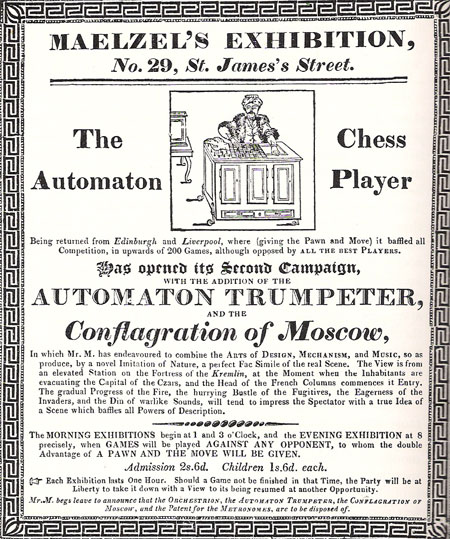
\includegraphics[width=\linewidth]{graphics/Henkin12.jpg}
  \caption{An advertisement for M\"alzel's appearance with the Mechanical Turk in London}
  \label{fig:turk}
\end{marginfigure}
A system of mirrors created the illusion that this table was transparent from all sides. Actually, a little hunchback who was an expert chess player sat inside and guided the puppet’s hand by means of strings. One can imagine a philosophical counterpart to this device. The puppet called ‘historical materialism’ is to win all the time. It can easily be a match for anyone if it enlists the services of theology, which today, as we know, is wizened and has to keep out of sight. 	


\section{II}

\newthought{`One of the most remarkable characteristics of human nature,'} writes Lotze, `is, alongside so much selfishness in specific instances, the freedom from envy which the present displays toward the future.' Reflection shows us that our image of happiness is thoroughly colored by the time to which the course of our own existence has assigned us. The kind of happiness that could arouse envy in us exists only in the air we have breathed, among people we could have talked to, women who could have given themselves to us. In other words, our image of happiness is indissolubly bound up with the image of redemption. The same applies to our view of the past, which is the concern of history. \begin{marginfigure}%
  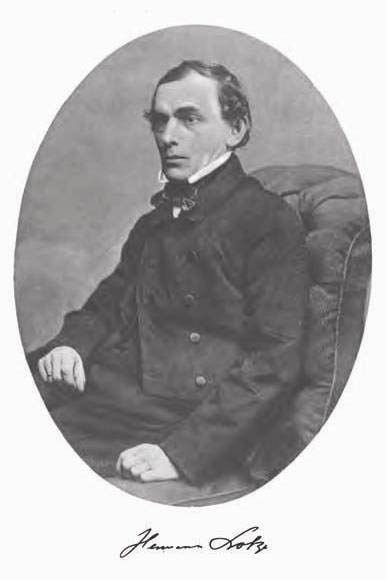
\includegraphics[width=\linewidth]{graphics/Lotze_Falckenberg1901.jpg}
  \caption{Rudolf Hermann Lotze (21 May 1817 – 1 July 1881)}
  \label{fig:Lotze}
\end{marginfigure}
The past carries with it a temporal index by which it is referred to redemption. There is a secret agreement between past generations and the present one. Our coming was expected on earth. Like every generation that preceded us, we have been endowed with a weak Messianic power, a power to which the past has a claim. That claim cannot be settled cheaply. Historical materialists are aware of that.	 


\section{III}

\newthought{A chronicler} who recites events without distinguishing between major and minor ones acts in accordance with the following truth: nothing that has ever happened should be regarded as lost for history. To be sure, only a redeemed mankind receives the fullness of its past-which is to say, only for a redeemed mankind has its past become citable in all its moments. Each moment it has lived becomes a citation a l'ordre du jour — and that day is Judgment Day.	 

\section{IV}	 
 	
%\marginnote{
%{\flushright \itshape	
\begin{quote}
Seek for food and clothing first, \\ then
the Kingdom of God shall be added unto you.\\
%}
-- Hegel, 1807\\
%}
\end{quote}
 	 	 
\newthought{The class struggle}, which is always present to a historian influenced by Marx, is a fight for the crude and material things without which no refined and spiritual things could exist. Nevertheless, it is not in the form of the spoils which fall to the victor that the latter make their presence felt in the class struggle. They manifest themselves in this struggle as courage, humor, cunning, and fortitude. They have retroactive force and will constantly call in question every victory, past and present, of the rulers. As flowers turn toward the sun, by dint of a secret heliotropism the past strives to turn toward that sun which is rising in the sky of history. A historical materialist must be aware of this most inconspicuous of all transformations.	 
 	 	 
\section{V}
\begin{marginfigure}%
  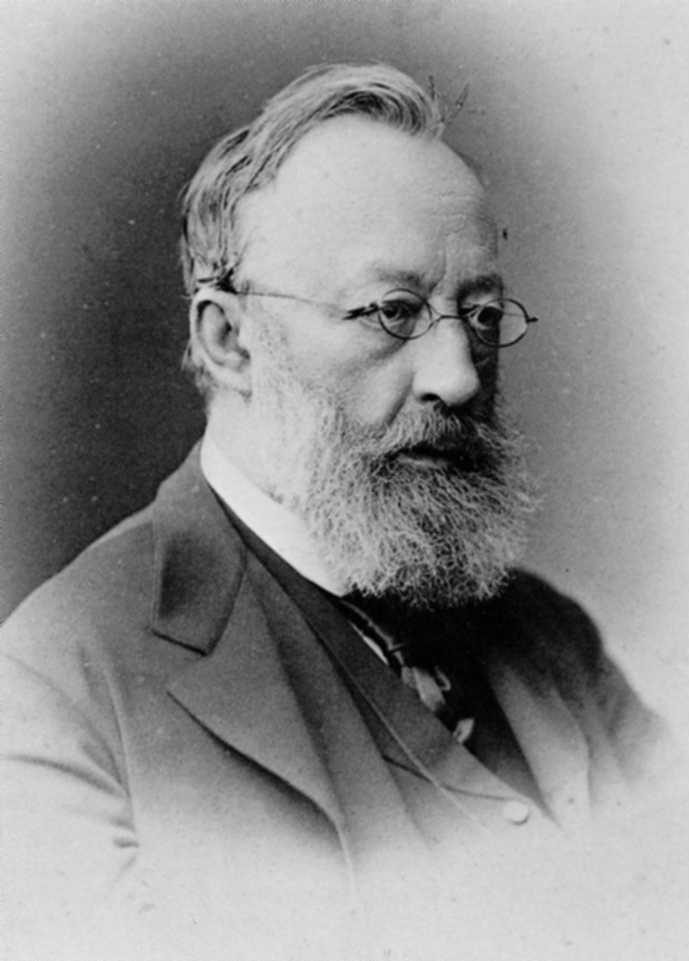
\includegraphics[width=\linewidth]{graphics/Johannes_Ganz_Gottfried_Keller_1885.jpg}
  \caption{Gottfried Keller (19 July 1819 – 15 July 1890)}
  \label{fig:Keller}
\end{marginfigure}
\newthought{The true picture} of the past flits by. The past can be seized only as an image which flashes up at the instant when it can be recognized and is never seen again. `The truth will not run away from us': in the historical outlook of historicism these words of Gottfried Keller mark the exact point where historical materialism cuts through historicism. 
For every image of the past that is not recognized by the present as one of its own concerns threatens to disappear irretrievably. (The good tidings which the historian of the past brings with throbbing heart may be lost in a void the very moment he opens his mouth.)	 

\newpage 	 	 
\section{VI} 	 
\newthought{To articulate the past} historically does not mean to recognize it `the way it really was' (Ranke). It means to seize hold of a memory as it flashes up at a moment of danger. 
Historical materialism wishes to retain that image of the past which unexpectedly appears to man singled out by history at a moment of danger. The danger affects both the content of the tradition and its receivers. The same threat hangs over both: that of becoming a tool of the ruling classes. 
\begin{marginfigure}%
  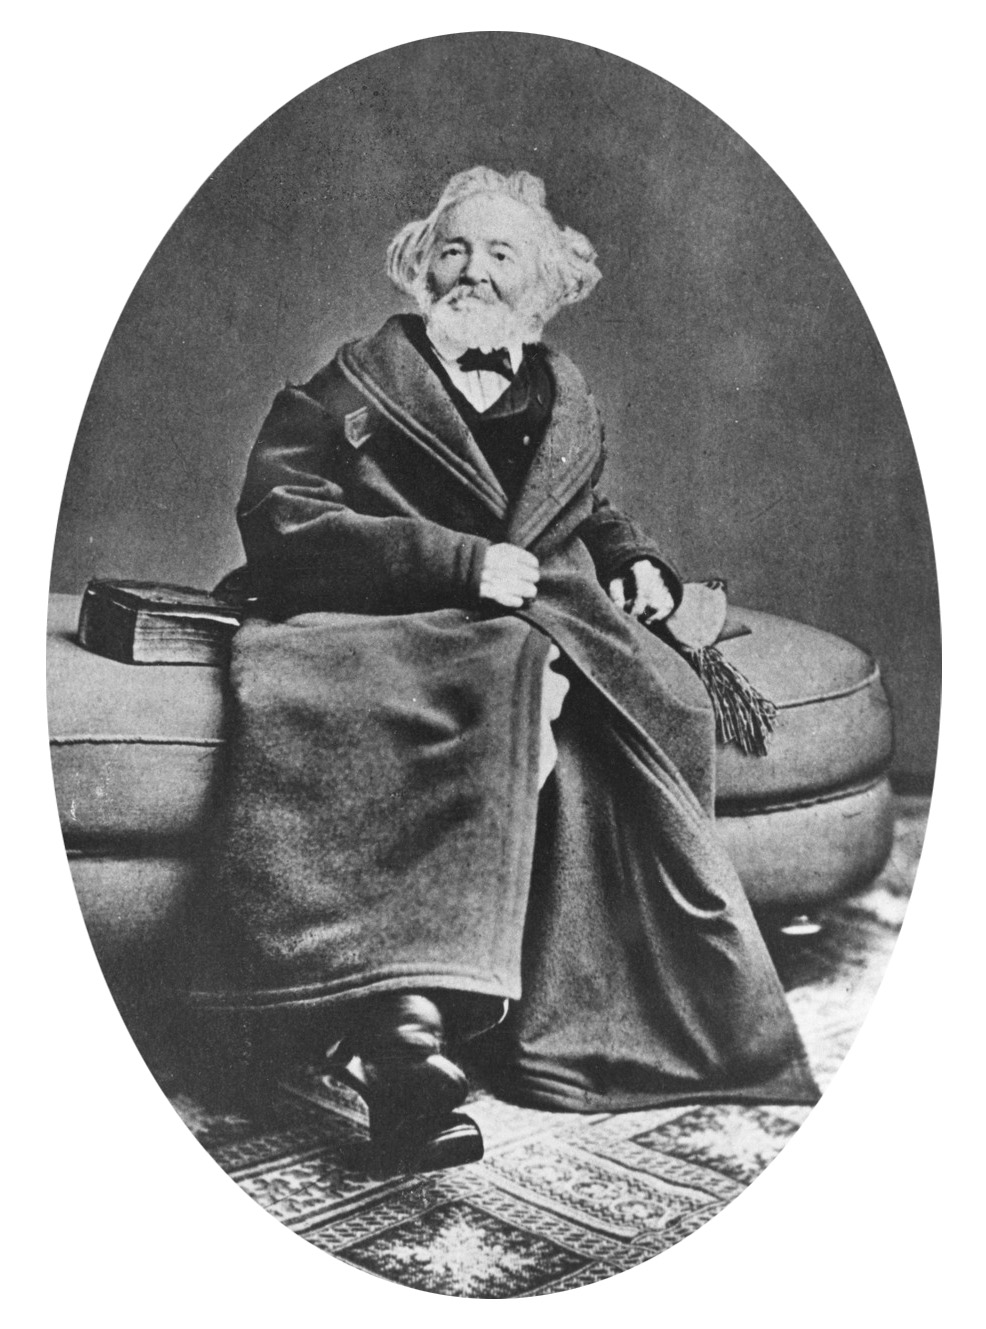
\includegraphics[width=\linewidth]{graphics/Leopold_Von_Ranke_1877.jpg}
  \caption{Leopold von Ranke (21 December 1795 – 23 May 1886)}
  \label{fig:Ranke}
\end{marginfigure}
In every era the attempt must be made anew to wrest tradition away from a conformism that is about to overpower it. The Messiah comes not only as the redeemer, he comes as the subduer of Antichrist. Only that historian will have the gift of fanning the spark of hope in the past who is firmly convinced that even the dead will not be safe from the enemy if he wins. And this enemy has not ceased to be victorious.	


\section{VII}	 
\begin{quote}
%\marginnote{
%{\flushright \itshape	
Consider the darkness and \\ the great cold
In this vale which \\ resounds with mystery.

%} 
%\vspace{10pt}

-- Brecht, \textit{The Threepenny Opera}
%} 
\end{quote}	 	 
\newthought{To historians} who wish to relive an era, Fustel de Coulanges recommends that they blot out everything they know about the later course of history. 
There is no better way of characterising the method with which historical materialism has broken. It is a process of empathy whose origin is the indolence of the heart, acedia, which despairs of grasping and holding the genuine historical image as it flares up briefly. Among medieval theologians it was regarded as the root cause of sadness.
\begin{marginfigure}%
  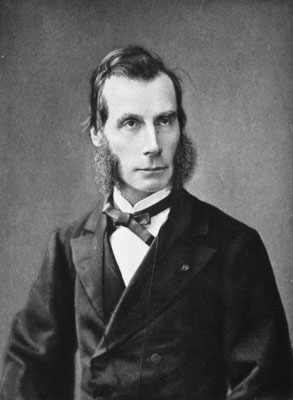
\includegraphics[width=\linewidth]{graphics/Numa_Fustel_de_Coulanges.jpg}
  \caption{Numa Denis Fustel de Coulanges (18 March 1830 – 12 September 1889) }
  \label{fig:deCoulanges}
\end{marginfigure}
Flaubert, who was familiar with it, wrote: `Peu de gens devineront combien il a fallu être triste pour ressusciter Carthage.'\footnote{`Few will be able to guess how sad one had to be in order to resuscitate Carthage.} The nature of this sadness stands out more clearly if one asks with whom the adherents of historicism actually empathize. The answer is inevitable: with the victor. 
And all rulers are the heirs of those who conquered before them. Hence, empathy with the victor invariably benefits the rulers. Historical materialists know what that means. Whoever has emerged victorious participates to this day in the triumphal procession in which the present rulers step over those who are lying prostrate. According to traditional practice, the spoils are carried along in the procession. They are called cultural treasures, and a historical materialist views them with cautious detachment. For without exception the cultural treasures he surveys have an origin which he cannot contemplate without horror. They owe their existence not only to the efforts of the great minds and talents who have created them, but also to the anonymous toil of their contemporaries. There is no document of civilization which is not at the same time a document of barbarism. And just as such a document is not free of barbarism, barbarism taints also the manner in which it was transmitted from one owner to another. A historical materialist therefore dissociates himself from it as far as possible. He regards it as his task to brush history against the grain. 	 
 	 	 
\section{VIII} 
\newthought{The tradition of the oppressed} teaches us that the `state of emergency' in which we live is not the exception but the rule. We must attain to a conception of history that is in keeping with this insight. Then we shall clearly realize that it is our task to bring about a real state of emergency, and this will improve our position in the struggle against Fascism. One reason why Fascism has a chance is that in the name of progress its opponents treat it as a historical norm. The current amazement that the things we are experiencing are `still' possible in the twentieth century is not philosophical. This amazement is not the beginning of knowledge—unless it is the knowledge that the view of history which gives rise to it is untenable.	

\section{IX}
\begin{marginfigure}%
  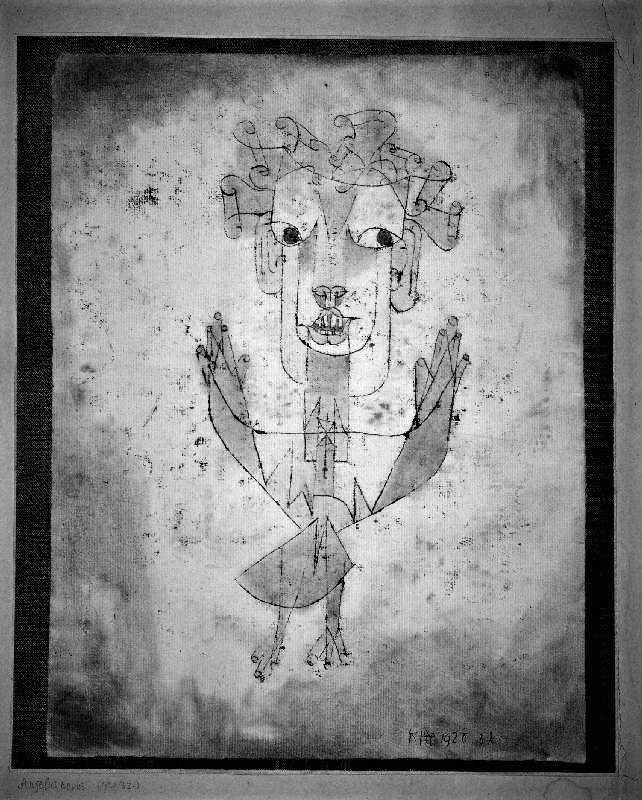
\includegraphics[width=\linewidth]{graphics/Klee,_paul,_angelus_novus,_1920.jpg}
  \caption{Angelus Novus (New Angel) by Paul Klee - The Israel Museum, Jerusalem}
  \label{fig:deCoulanges}
\end{marginfigure}
\begin{quote}
%% \marginnote{
%%{\flushright \itshape	
My wing is ready for flight, \\ 
I would like to turn back.If I stayed timeless \\time, 
I would have little luck. \\
 
%%\vspace{12pt}
 
Mein Flügel ist zum Schwung bereit,\\
ich kehrte gern zurück,\\
denn blieb ich auch lebendige Zeit,\\
ich hätte wenig Glück.\\

%%} 
%%\vspace{10pt}
-- Gerherd Scholem, \textit{Gruss vom Angelus}
%%} 
\end{quote} 	
 

\newthought{A Klee painting} named `Angelus Novus' shows an angel looking as though he is about to move away from something he is fixedly contemplating. His eyes are staring, his mouth is open, his wings are spread. This is how one pictures the angel of history. His face is turned toward the past. Where we perceive a chain of events, he sees one single catastrophe which keeps piling wreckage and hurls it in front of his feet. The angel would like to stay, awaken the dead, and make whole what has been smashed. But a storm is blowing in from Paradise; it has got caught in his wings with such a violence that the angel can no longer close them. The storm irresistibly propels him into the future to which his back is turned, while the pile of debris before him grows skyward. This storm is what we call progress. 
 
\section{X}	 
 	 	 
\newthought{The themes} which monastic discipline assigned to friars for meditation were designed to turn them away from the world and its affairs. The thoughts which we are developing here originate from similar considerations. At a moment when the politicians in whom the opponents of Fascism had placed their hopes are prostrate and confirm their defeat by betraying their own cause, these observations are intended to disintangle the political worldlings from the snares in which the traitors have entrapped them. Our consideration proceeds from the insight that the politicians’ stubborn faith in progress, their confidence in their `mass basis', and, finally, their servile integration in an uncontrollable apparatus have been three aspects of the same thing. It seeks to convey an idea of the high price our accustomed thinking will have to pay for a conception of history that avoids any complicity with the thinking to which these politicians continue to adhere.	 
 	 	 
\section{XI}	 
 	 	 
\newthought{The conformism} which has been part and parcel of Social Democracy from the beginning attaches not only to its political tactics but to its economic views as well. It is one reason for its later breakdown. Nothing has corrupted the German working, class so much as the notion that it was moving, with the current. It regarded technological developments as the fall of the stream with which it thought it was moving. From there it was but a step to the illusion that the factory work which was supposed to tend toward technological progress constituted a political achievement. The old Protestant ethics of work was resurrected among German workers in secularized form. The Gotha Program \footnote{The Gotha Congress of 1875 'United the two German Socialist parties, one led by Ferdinand Lassalle, the other by Karl Marx and Wilhelm Liebknecht. The program, drafted by Liebknecht and Lassalle, was severely attacked by Marx in London. See his `Critique of the Gotha Program'} already bears traces of this confusion, defining labor as `the source of all wealth and all culture.' Smelling a rat, Marx countered that `\ldots the man who possesses no other property than his labor power' must of necessity become `the slave of other men who have made themselves the owners\ldots' However, the confusion spread, and soon thereafter Josef Dietzgen proclaimed: `The savior of modern times is called work. The \ldots improvement\ldots of labor constitutes the wealth which is now able to accomplish what no redeemer has ever been able to do.' This vulgar-Marxist conception of the nature of labor bypasses the question of how its products might benefit the workers while still not being at, their disposal. It recognizes only the progress in the mastery of nature, not the retrogression of society; it already displays the technocratic features later encountered in Fascism. Among these is a conception of nature which differs ominously from the one in the Socialist utopias before the 1848 revolution. The new conception of labor amounts to the exploitation of nature, which with naive complacency is contrasted with the exploitation of the proletariat. Compared with this positivistic conception, Fourier's fantasies, which have so often been ridiculed, prove to be surprisingly sound. According to Fourier, as a result of efficient cooperative labor, four moons would illuminate the earthly night, the ice would recede from the poles, sea water would no longer taste salty, and beasts of prey would do man's bidding. All this illustrates a kind of labor which, far from exploiting nature, is capable of delivering her of the creations which lie dormant in her womb as potentials. Nature, which, as Dietzgen puts it, `exists gratis,' is a complement to the corrupted conception of labor.	 
 	 		
\section{XVII}	 
 	 	 
\newthought{Historicism rightly} culminates in universal history. Materialistic historiography differs from it as to method more clearly than from any other kind. Universal history has no theoretical armature. Its method is additive; it musters a mass of data to fill the homogoneous, empty time. Materialistic historiography, on the other hand, is based on a constructive principle. Thinking involves not only the flow of thoughts, but their arrest as well. Where thinking suddenly stops in a configuration pregnant with tensions, it gives that configuration a shock, by which it cristallizes into a monad. A historical materialist approaches a historical subject only where he encountes it as a monad. In this structure he recognizes the sign of a Messianic cessation of happening, or, put differently, a revolutionary chance in the fight for the oppressed past. He takes cognizance of it in order to blast a specific era out of the homogenous course of history—blasting a specific life out of the era or a specific work out of the lifework. As a result of this method the lifework is preserved in this work and at the same time canceled\footnote{The Hegelian term \textit{aufheben} in its threefold meaning: to preserve, to elevate, to cancel.}; in the lifework, the era; and in the era, the entire course of history. The nourishing fruit of the historically understood contains time as a precious but tasteless seed. 	 
 	 	  
\section{XVIII}	 
 	 	 
\newthought{`In relation} to the history of organic life on earth,' writes a modem biologist, `the paltry fifty millennia of homo sapiens constitute something like two seconds at the close of a twenty-four-hour day. On this scale, the history of civilized mankind would fill one-fifth of the last second of the last hour.' The present, which, as a model of Messianic time, comprises the entire history of mankind in an enormous abridgment, coincides exactly with the stature which the history of mankind has in the universe.	 
 	 	 
 	 	 
\subsection{A}	 
 	 	 
\newthought{Historicism contents} itself with establishing a causal connection between various moments in history. But no fact that is a cause is for that very reason historical. It became historical posthumously, as it were, though events that may be separated from it by thousands of years. A historian who takes this as his point of departure stops telling the sequence of events like the beads of a rosary. Instead, he grasps the constellation which his own era has formed with a definite earlier one. Thus he establishes a conception of the present as the `time of the now' which is shot through with chips of Messianic time.	 
 	 	 
\subsection{B}	 
 	 	 
\newthought{The soothsayers} who found out from time what it had in store certainly did not experience time as either homogeneous or empty. Anyone who keeps this in mind will perhaps get an idea of how past times were experienced in remembrance--namely, in just the same way. We know that the Jews were prohibited from investigating the future. The Torah and the prayers instruct them in remembrance, however. This stripped the future of its magic, to which all those succumb who turn to the soothsayers for enlightenment. This does not imply, however, that for the Jews the future turned into homogeneous, empty time. For every second of time was the strait gate through which Messiah might enter.	 

\nocite{*}
{\footnotesize
\bibliographystyle{plain}
\bibliography{references}
}
\end{document}
